\chapter{Liquidit�tsplan}

\begin{figure}[htbp]
  \centering
     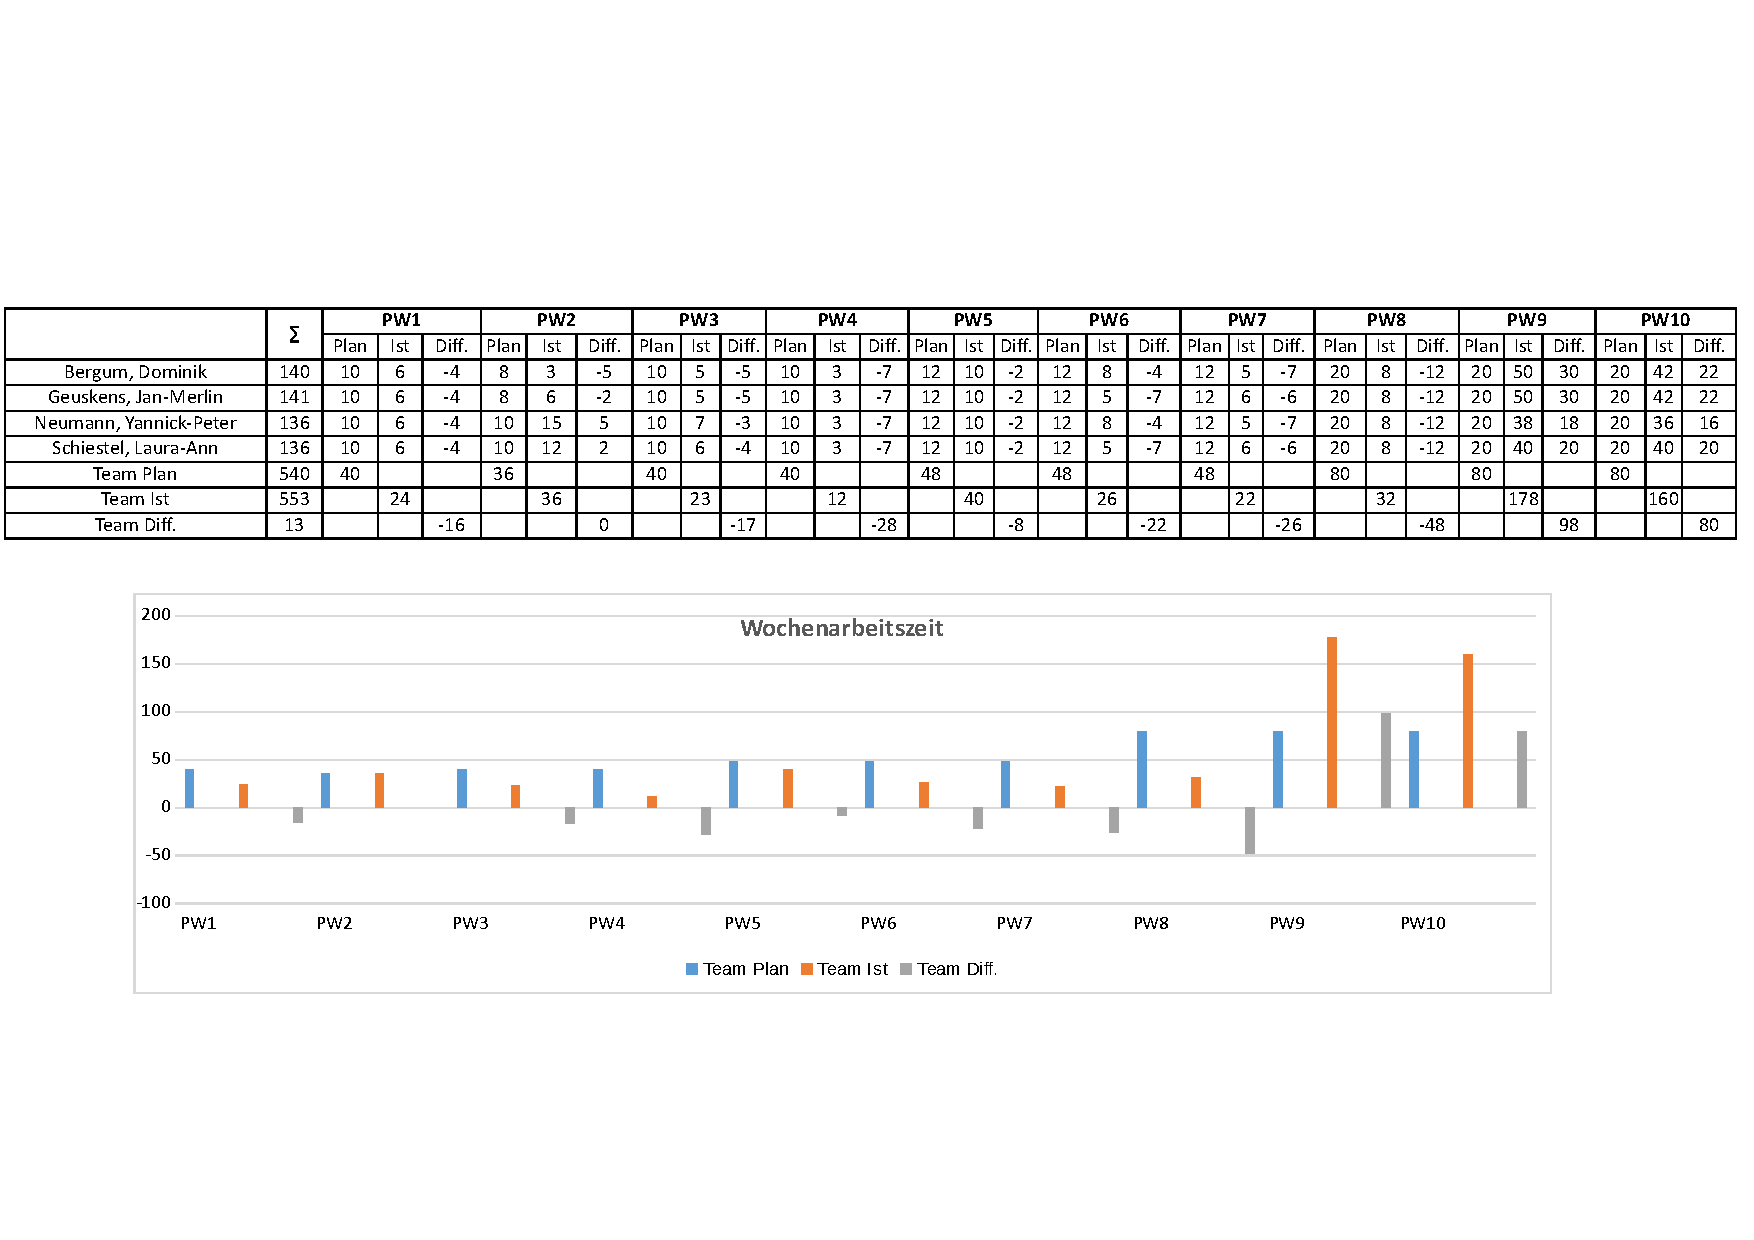
\includegraphics[keepaspectratio=true,scale=0.61,angle={90}]{Graphics/Liquid1.pdf}
  \caption{Liquidit�tsplan}
  \label{fig:Liquid}
\end{figure}

\clearpage
Der Liquidit�tsplan aus \ref{fig:Liquid} stellt die Arbeitszeiten der einzelnen
Teammitglieder, sowohl die geplanten als auch die tats�chlichen Stunden, dar.
\newline
Der Planung liegen ca. 540 Stunden zu Grunde (135 pro Teammitglied). Die
tats�chliche Arbeitszeit fiel unwesentlich h�her aus.
\newline
Eine Abweichung zwischen Soll- und Ist-Zeiten ist bei allen
Teammitgliedern zu erkennen. Dies ist unterschiedlichen Gr�nden geschuldet.
Beispielsweise variierte die Einarbeitungszeit In Unity und Blender bei den
Teammitgliedern stark, da die Kenntnisst�nde unterschiedlich waren. Auch die
Fehleinsch�tzung des Aufwands der unterschiedlichen Arbeitspaketen ist ein
Grund f�r die Abweichung. Desweiteren beanspruchte auch der
telekommunikationsspezifische Teil des Praktikum mehr Zeit als erwartet,
wodurch die Soll-Zeiten in den Projektwochen 3-4 und 7-8 nicht erf�llt wurden.
